% ---- pg-350 （书页 338） ----

考虑从多元正态随机变量导出的主成分, 会提供大量信息. 设 $\mathbf{X}$ 的分布为 $N_p(\boldsymbol{\mu},\boldsymbol{\Sigma})$. 我们从\hyperref[eq:4-7]{式(4-7)}知道, 在以 $\boldsymbol{\mu}$ 为中心的椭球上, $\mathbf{X}$ 的密度是常数
\[
(\mathbf{x}-\boldsymbol{\mu})'\boldsymbol{\Sigma}^{-1}(\mathbf{x}-\boldsymbol{\mu})=c^2
\]
其轴为 $\pm c\sqrt{\lambda_i}\mathbf{e}_i, i=1,2,\cdots,p$, 其中 $(\lambda_i,\mathbf{e}_i)$ 是 $\boldsymbol{\Sigma}$ 的特征值-特征向量对. 在原点为 $\boldsymbol{\mu}$、坐标轴平行于原坐标轴 $x_1,x_2,\cdots,x_p$ 的坐标系中, 位于椭球第 $i$ 条坐标轴上的一点, 将有与 $\mathbf{e}_i'=[e_{i1},e_{i2},\cdots,e_{ip}]$ 成比例的坐标. 在下面的讨论中, 令 $\boldsymbol{\mu}=\mathbf{0}$ 是方便的.\footnote{{\footnotesize 这样做可不失一般性, 因为总可以将正态向量 $\mathbf{X}$ 变换为正态向量 $\mathbf{W}=\mathbf{X}-\boldsymbol{\mu}$ 而有 $E(\mathbf{W})=0$, 而 $\mathrm{Cov}(\mathbf{X})=\mathrm{Cov}(\mathbf{W})$.}}

从 2.3 节的讨论, 取 $\boldsymbol{A}=\boldsymbol{\Sigma}^{-1}$, 我们可有
\[
c^2=\mathbf{x}'\boldsymbol{\Sigma}^{-1}\mathbf{x}=\frac{1}{\lambda_1}(\mathbf{e}_1'\mathbf{x})^2+\frac{1}{\lambda_2}(\mathbf{e}_2'\mathbf{x})^2+\cdots+\frac{1}{\lambda_p}(\mathbf{e}_p'\mathbf{x})^2
\]
其中 $\mathbf{e}_1'\mathbf{x},\mathbf{e}_2'\mathbf{x},\cdots,\mathbf{e}_p'\mathbf{x}$ 为 $\mathbf{x}$ 的主成分. 设 $y_1=\mathbf{e}_1'\mathbf{x}, y_2=\mathbf{e}_2'\mathbf{x},\cdots,y_p=\mathbf{e}_p'\mathbf{x}$, 我们有
\[
c^2=\frac{1}{\lambda_1}y_1^2+\frac{1}{\lambda_2}y_2^2+\cdots+\frac{1}{\lambda_p}y_p^2
\]
并且在具有分别沿 $\mathbf{e}_1,\mathbf{e}_2,\cdots,\mathbf{e}_p$ 方向的坐标轴为 $y_1,y_2,\cdots,y_p$ 的坐标系中, 上式定义了一个椭球(由于 $\lambda_1,\lambda_2,\cdots,\lambda_p$ 都是正的). 如果 $\lambda_1$ 是最大的特征值, 那么主轴沿着 $\mathbf{e}_1$ 的方向. 余下较次要的坐标轴沿着由 $\mathbf{e}_1,\cdots,\mathbf{e}_p$ 确定的方向.

总而言之, 主成分 $y_1=\mathbf{e}_1'\mathbf{x}, y_2=\mathbf{e}_2'\mathbf{x},\cdots,y_p=\mathbf{e}_p'\mathbf{x}$ 沿着常数密度椭球的坐标轴方向. 因此, 在第 $i$ 条椭球轴上任一点 $\mathbf{x}$ 的坐标, 与 $\mathbf{e}_i'=[e_{i1},e_{i2},\cdots,e_{ip}]$ 成比例, 并且还必定有形如 $[0,\cdots,0,y_i,0,\cdots,0]$ 的主成分.

当 $\boldsymbol{\mu}\neq\mathbf{0}$ 时, 均值中心化主成分 $y_i=\mathbf{e}_i'(\mathbf{x}-\boldsymbol{\mu})$ 的均值为 0, 且在 $\mathbf{e}_i$ 的方向上.

\hyperref[fig:8.1]{图 8.1} 表示的是一个均值 $\boldsymbol{\mu}=\mathbf{0}$ 和 $\rho=0.75$ 的二元正态随机向量的常数密度椭圆和主成分. 我们看到, 将原坐标轴旋转一个角度 $\theta$, 直到它们与常数密度椭圆的轴重合, 就得到主成分. 这个结论对 $p>2$ 维时同样成立.

\begin{mvfigure}
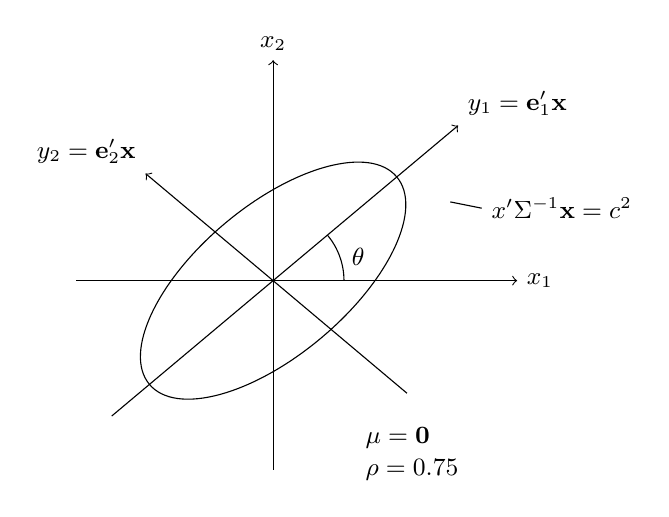
\begin{tikzpicture}[scale=1.0]
\draw[->] (-2.5,0) -- (3.1,0) node[right,font=\small] {$x_1$};
\draw[->] (0,-2.4) -- (0,2.8) node[above,font=\small] {$x_2$};
% 主成分轴 y1、y2 及其反向延长线
\draw (0,0) -- (-2.05,-1.72);
\draw[->] (0,0) -- (2.35,1.97);
\node[above right,font=\small] at (2.35,1.97) {$y_1=\mathbf{e}_1'\mathbf{x}$};
\draw (0,0) -- (1.70,-1.43);
\draw[->] (0,0) -- (-1.62,1.36);
\node[above left,font=\small] at (-1.62,1.36) {$y_2=\mathbf{e}_2'\mathbf{x}$};
% 常数密度椭圆
\draw[rotate=40] (0,0) ellipse (2.05 and 0.95);
% 旋转角 theta
\draw (0.9,0) arc (0:40:0.9);
\node[font=\small] at (1.08,0.30) {$\theta$};
% 标注
\draw (2.25,1.00) -- (2.65,0.92);
\node[right,font=\small] at (2.65,0.92) {$x'\boldsymbol{\Sigma}^{-1}\mathbf{x}=c^2$};
\node[right,font=\small] at (1.05,-2.00) {$\boldsymbol{\mu}=\mathbf{0}$};
\node[right,font=\small] at (1.05,-2.40) {$\rho=0.75$};
\end{tikzpicture}
\phantomsection\label{fig:8.1}\mvcap{图 8.1\quad 均值为 $\mathbf{0}$ 的二元正态随机向量 $\mathbf{X}$, 其常数密度椭圆 $\mathbf{x}'\boldsymbol{\Sigma}^{-1}\mathbf{x}=c^2$ 和主成分 $y_1,y_2$}
\end{mvfigure}

\mvsub{从标准化变量得到的主成分}

主成分也可以从标准化变量
\phantomsection\label{eq:8-9}
\begin{equation}
\begin{aligned}
Z_1&=\frac{(X_1-\mu_1)}{\sqrt{\sigma_{11}}}\\
Z_2&=\frac{(X_2-\mu_2)}{\sqrt{\sigma_{22}}}\\
&\vdots\\
Z_p&=\frac{(X_p-\mu_p)}{\sqrt{\sigma_{pp}}}
\end{aligned}
\tag{8-9}
\end{equation}
得到. 采用矩阵记号
